\documentclass[letterpaper, reqno,11pt]{article}
\usepackage[margin=1.0in]{geometry}
\usepackage{color,latexsym,amsmath,amssymb,graphicx,float,listings,tikz,xcolor}
\usepackage{hyperref}

\hypersetup{
colorlinks=true,
linkcolor=magenta,
filecolor=magenta,
urlcolor=cyan,
}

\lstset{
basicstyle=\ttfamily,
columns=fullflexible,
frame=single,
breaklines=true,
postbreak=\mbox{\textcolor{red}{$\hookrightarrow$}\space},
}

\graphicspath{ {images/} }

\begin{document}

\begin{titlepage}
\newgeometry{margin=3cm}
\centering

\vspace*{\stretch{2}}

\Large Investigation of HeNe Laser Properties

\normalsize

\vspace{\stretch{1}}

% \normalsize Power Supplies and Voltage Regulators

\vspace{\stretch{0.5}}

\begin{tabular}{ll}
Name & Xander Naumenko \\[2ex]
Student number & 38198354 \\[2ex]
Partner & Renu Rajamagesh \\[2ex]
Lab name & Fourier optics \\[2ex]
Lab station  & L2C \\[2ex]
Assigned TA            & Rachel Wang, Mahdi Rabiel \\[2ex]
Lab \#            & 2 \\[2ex]
Notes &  N/A
\end{tabular}

\vspace{\stretch{1}}

\begin{abstract}
    HeNe lasers are one relatively easy way of creating a laser beam for general optics uses. In this lab we investigate the properties and operating conditions of such lasers. Specifically, the stability conditions of the lasing and the spectral emissions of the HeNe were analyzed thoroughly to get a clear picture of the underlying mechanics causing the laser's production. The biggest result is that, using an op-amp, the spectral difference between lasing and non-lasing HeNe was recorded to have peaks at the atomic frequencies of the laser.
\end{abstract}

\vspace{\stretch{2}}
\end{titlepage}

\newpage

\section{Research Note}

\subsection{Introduction}

\newpage

\section{2.3.1: Laser Alignment and Stability}

\noindent \textcolor{red}{2.3.1A.} The stability conditions for lasing, as described in the appendix are:
\[
0\leq \left(1+ \frac{d}{R_1}\right) \left( 1+ \frac{d}{R_2} \right) \leq 1
.\]
In our case, $R_2=\infty$, so this reduces to $0\leq 1+ \frac{d}{R_1}\leq 1$. Assuming $R_1$ is concave (so $R_1< 0$), this gives $d=-R_1$.

To measure this, we first got the HeNe lasing by adjusting the mirror as described in the manual. Then we pushed the mirror back until lasing stopped, and measured the distance from the fixed HR mirror. Experimentally we found this to be $53$cm, so $R_2=-53$cm.

\medskip

\noindent \textcolor{red}{2.3.1B.} With the new mirror, there were four regions (all distances measured relative to HR mirror): at less than 54cm there was lasing, between 54cm and 56.5cm there was none, between 56.5cm and 65cm it lased and then finally disappeared after 65cm. However after 65cm it wasn't entirely consistent, and depending on fine alignment it would sometimes lase farther than that.

These points can be explained theoretically. The first disappearance corresponds to $1+\frac{d}{R_1}=0$, i.e. $d=-R_1$. From part A we'd expect this to be around $53$cm, which our measurement of $54$cm was fairly close to. The reappearance at $56.5$ is for $1+\frac{d}{R_2}=0\implies d=-R_2$. From the box the mirror came in we expect this to be $60$cm. One possible reason for this somewhat small discrepancy is just the measurement error, as using a meter stick to estimate exactly where the laser starts can be inconsistent. The final reappearance occurs when
\[
\left(1+ \frac{d}{R_1}\right) \left( 1+ \frac{d}{R_2} \right) = 1\implies d=-(R_1+R_2)
.\]
Our measured value was 65cm, which was very difference than the expected of 113. In fact, given where the raspberry pi camera was located and the length of the slide we shouldn't have even seen a reappearance at all. The most likely cause for this discrepancy is misalignment of the mirrors. Even if everything else in the setup was perfect, the mirrors have finite size, so a small misalignment could cause the reflected laser to strike outside the mirror when distances are far enough. Something like alignment would also explain the inconsistencies with seeing exactly where the laser reappears. See figure \ref{fig:1A} for the plot and table.

\begin{figure}[htpb]
    \centering
    \begin{minipage}[b]{0.45\textwidth}
    \begin{tabular}{|l|l|l|}
    \hline
    Value & Theoretical & Measured \\
    \hline
    $-R_1$ & 53 & 54 \\
    $-R_2$ & 60 & 56.5 \\
    $-(R_1+R_2)$ & 113 & 65 \\
    \hline
    \end{tabular}
    \caption{Table caption.}
    \label{fig:table1}
    \end{minipage}
    \hfill
    % \includegraphics[width=0.8\text width]{1A}
    \caption{Plot and table for 2.3.1B. The theoretical values were found from 2.3.1B and the mirror box.}
    \label{fig:1A}
\end{figure}

\noindent \textcolor{blue}{2.3.1i.} You could use a convex mirror, for the calculations let's say for $R_2$ while $R_1$ is still concave. From the condition that $\left(1+ \frac{d}{R_1}\right) \left( 1+ \frac{d}{R_2} \right)\geq 0$ we have that $d<R_1$. From the condition that $\left(1+ \frac{d}{R_1}\right) \left( 1+ \frac{d}{R_2} \right)\leq 1$, we have that $-R_1<R_2$, i.e. the magnitude of the convex mirror's radius of curvature must be greater than that of the concave mirror.

\noindent \textcolor{red}{2.3.2A.} See figure \ref{fig:2A} for some of the observed nodes. The highest order node observed was Hermite-Gaussian TEM$_{22}$, see the figure for explanations.

\begin{figure}[tb]
    \centering
    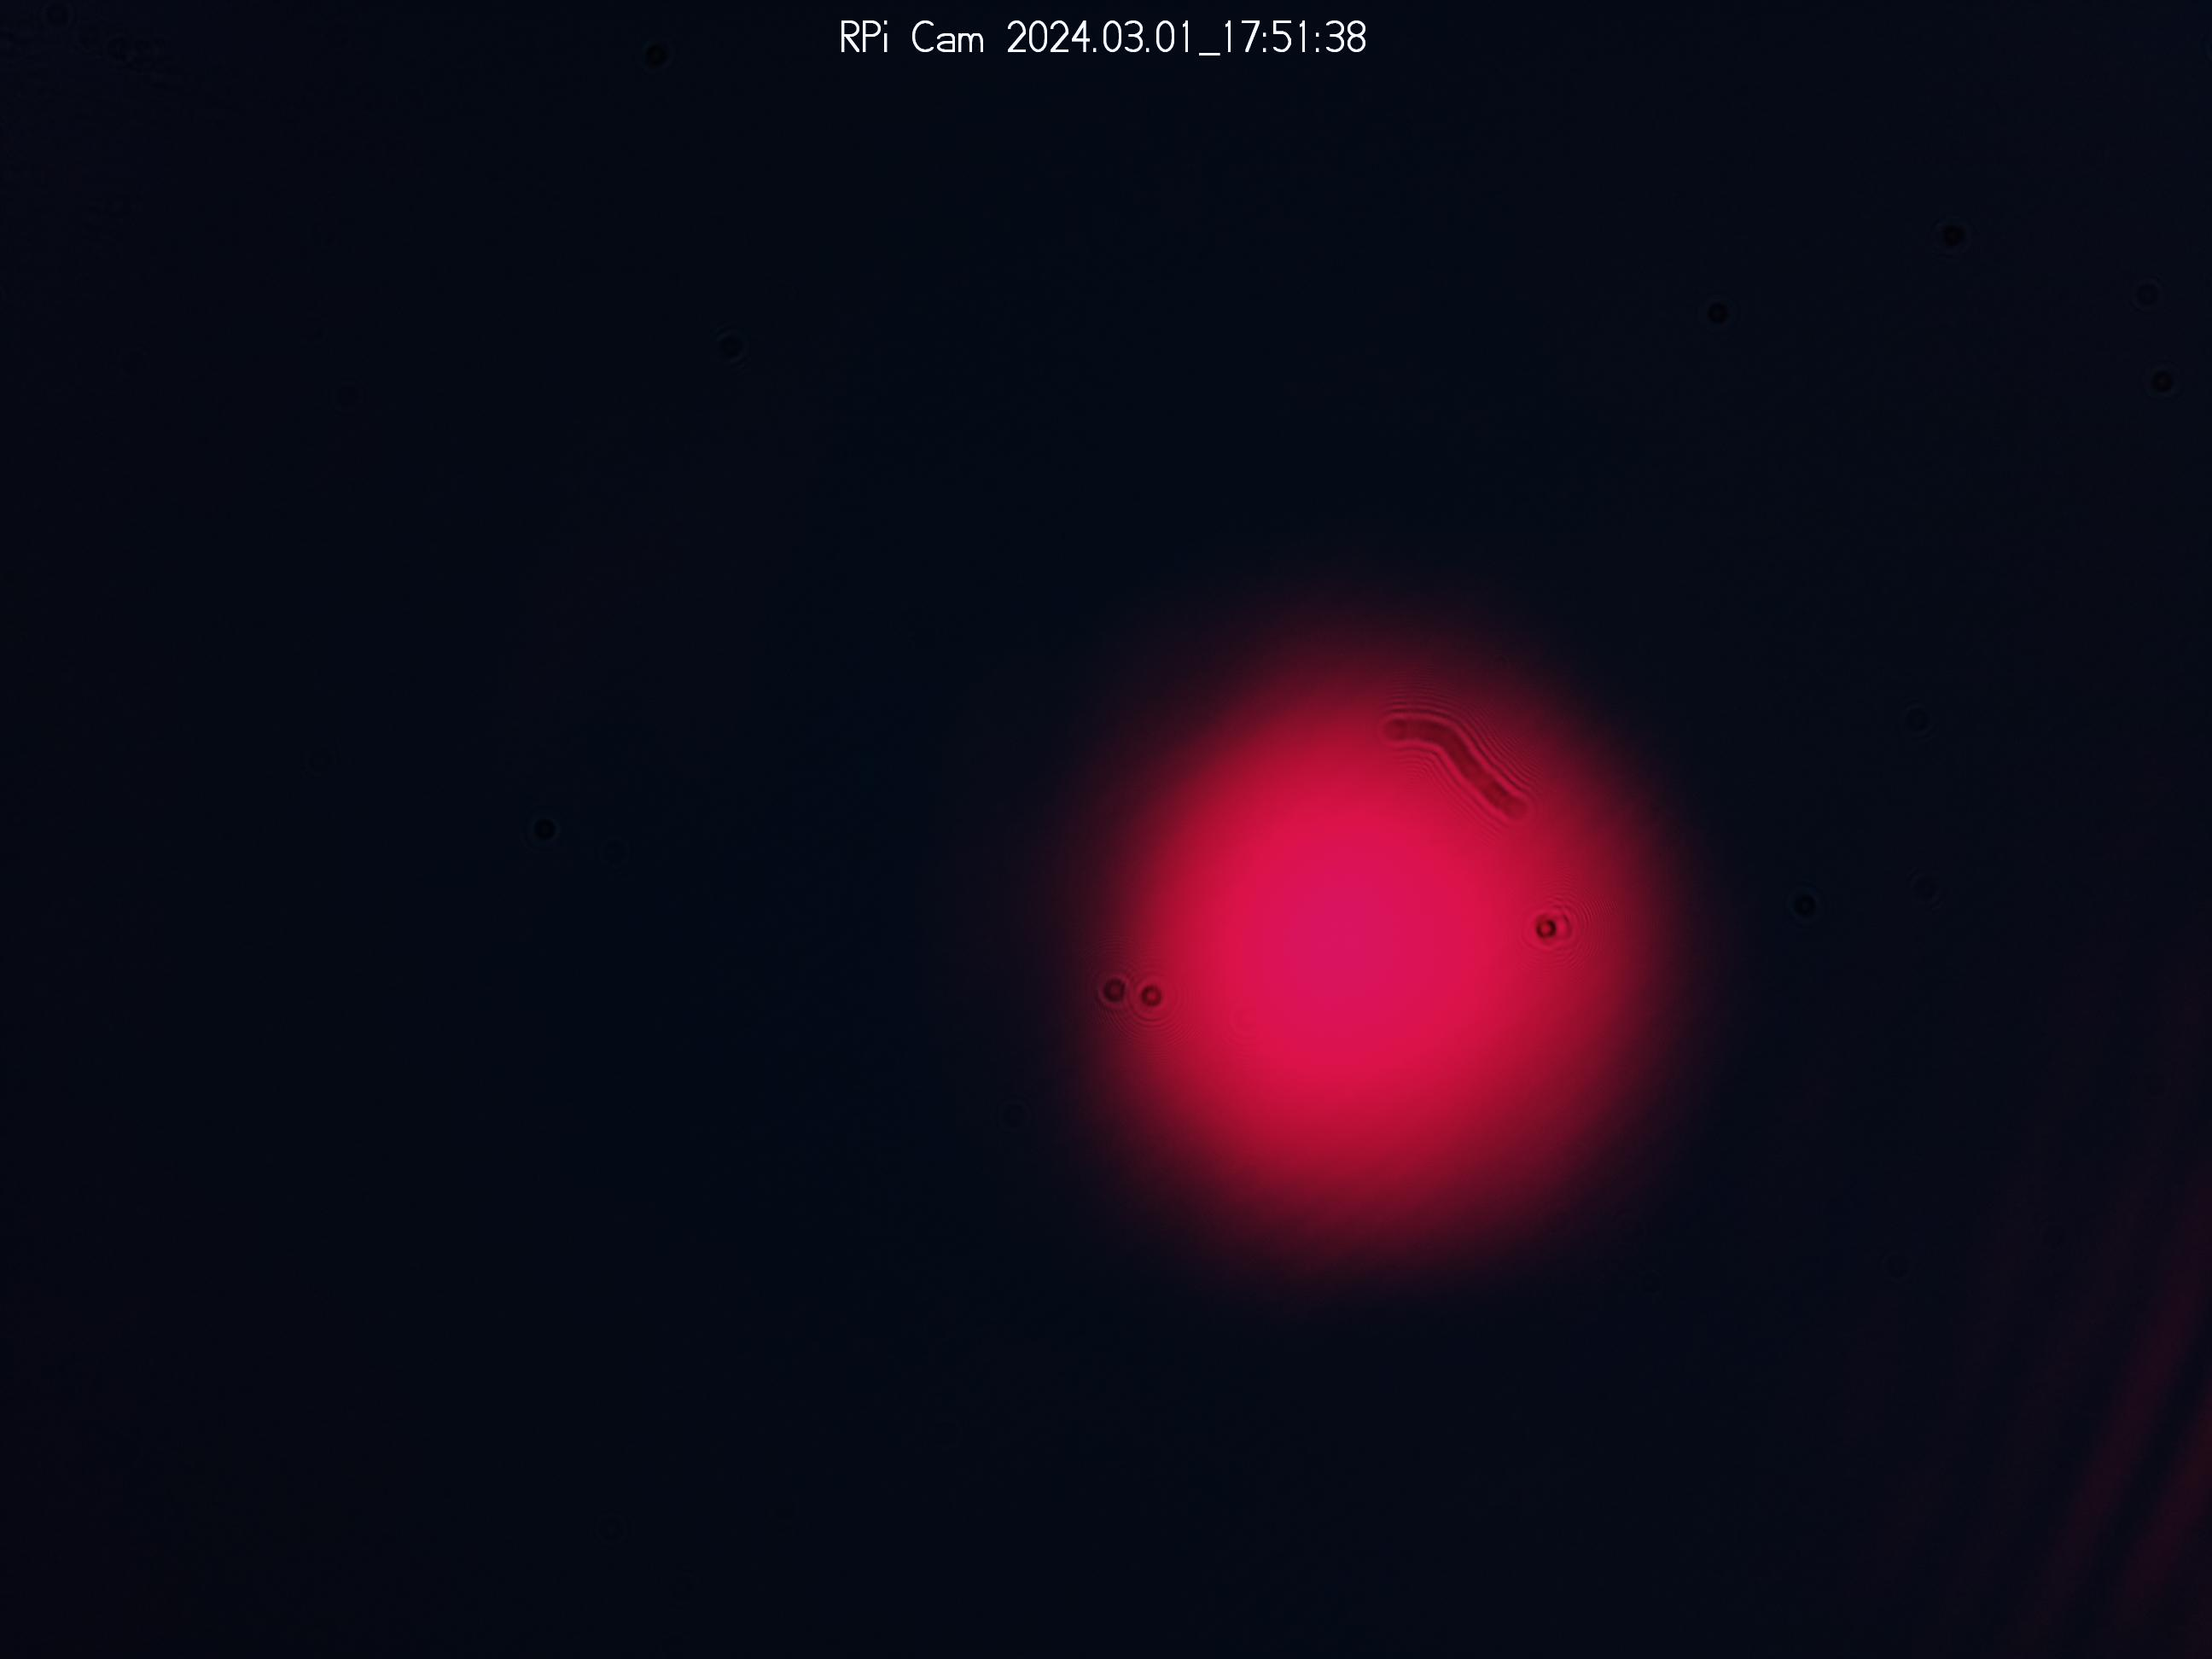
\includegraphics[width=0.3\textwidth]{data/2A/im_0228_20240301_175138.jpg}
    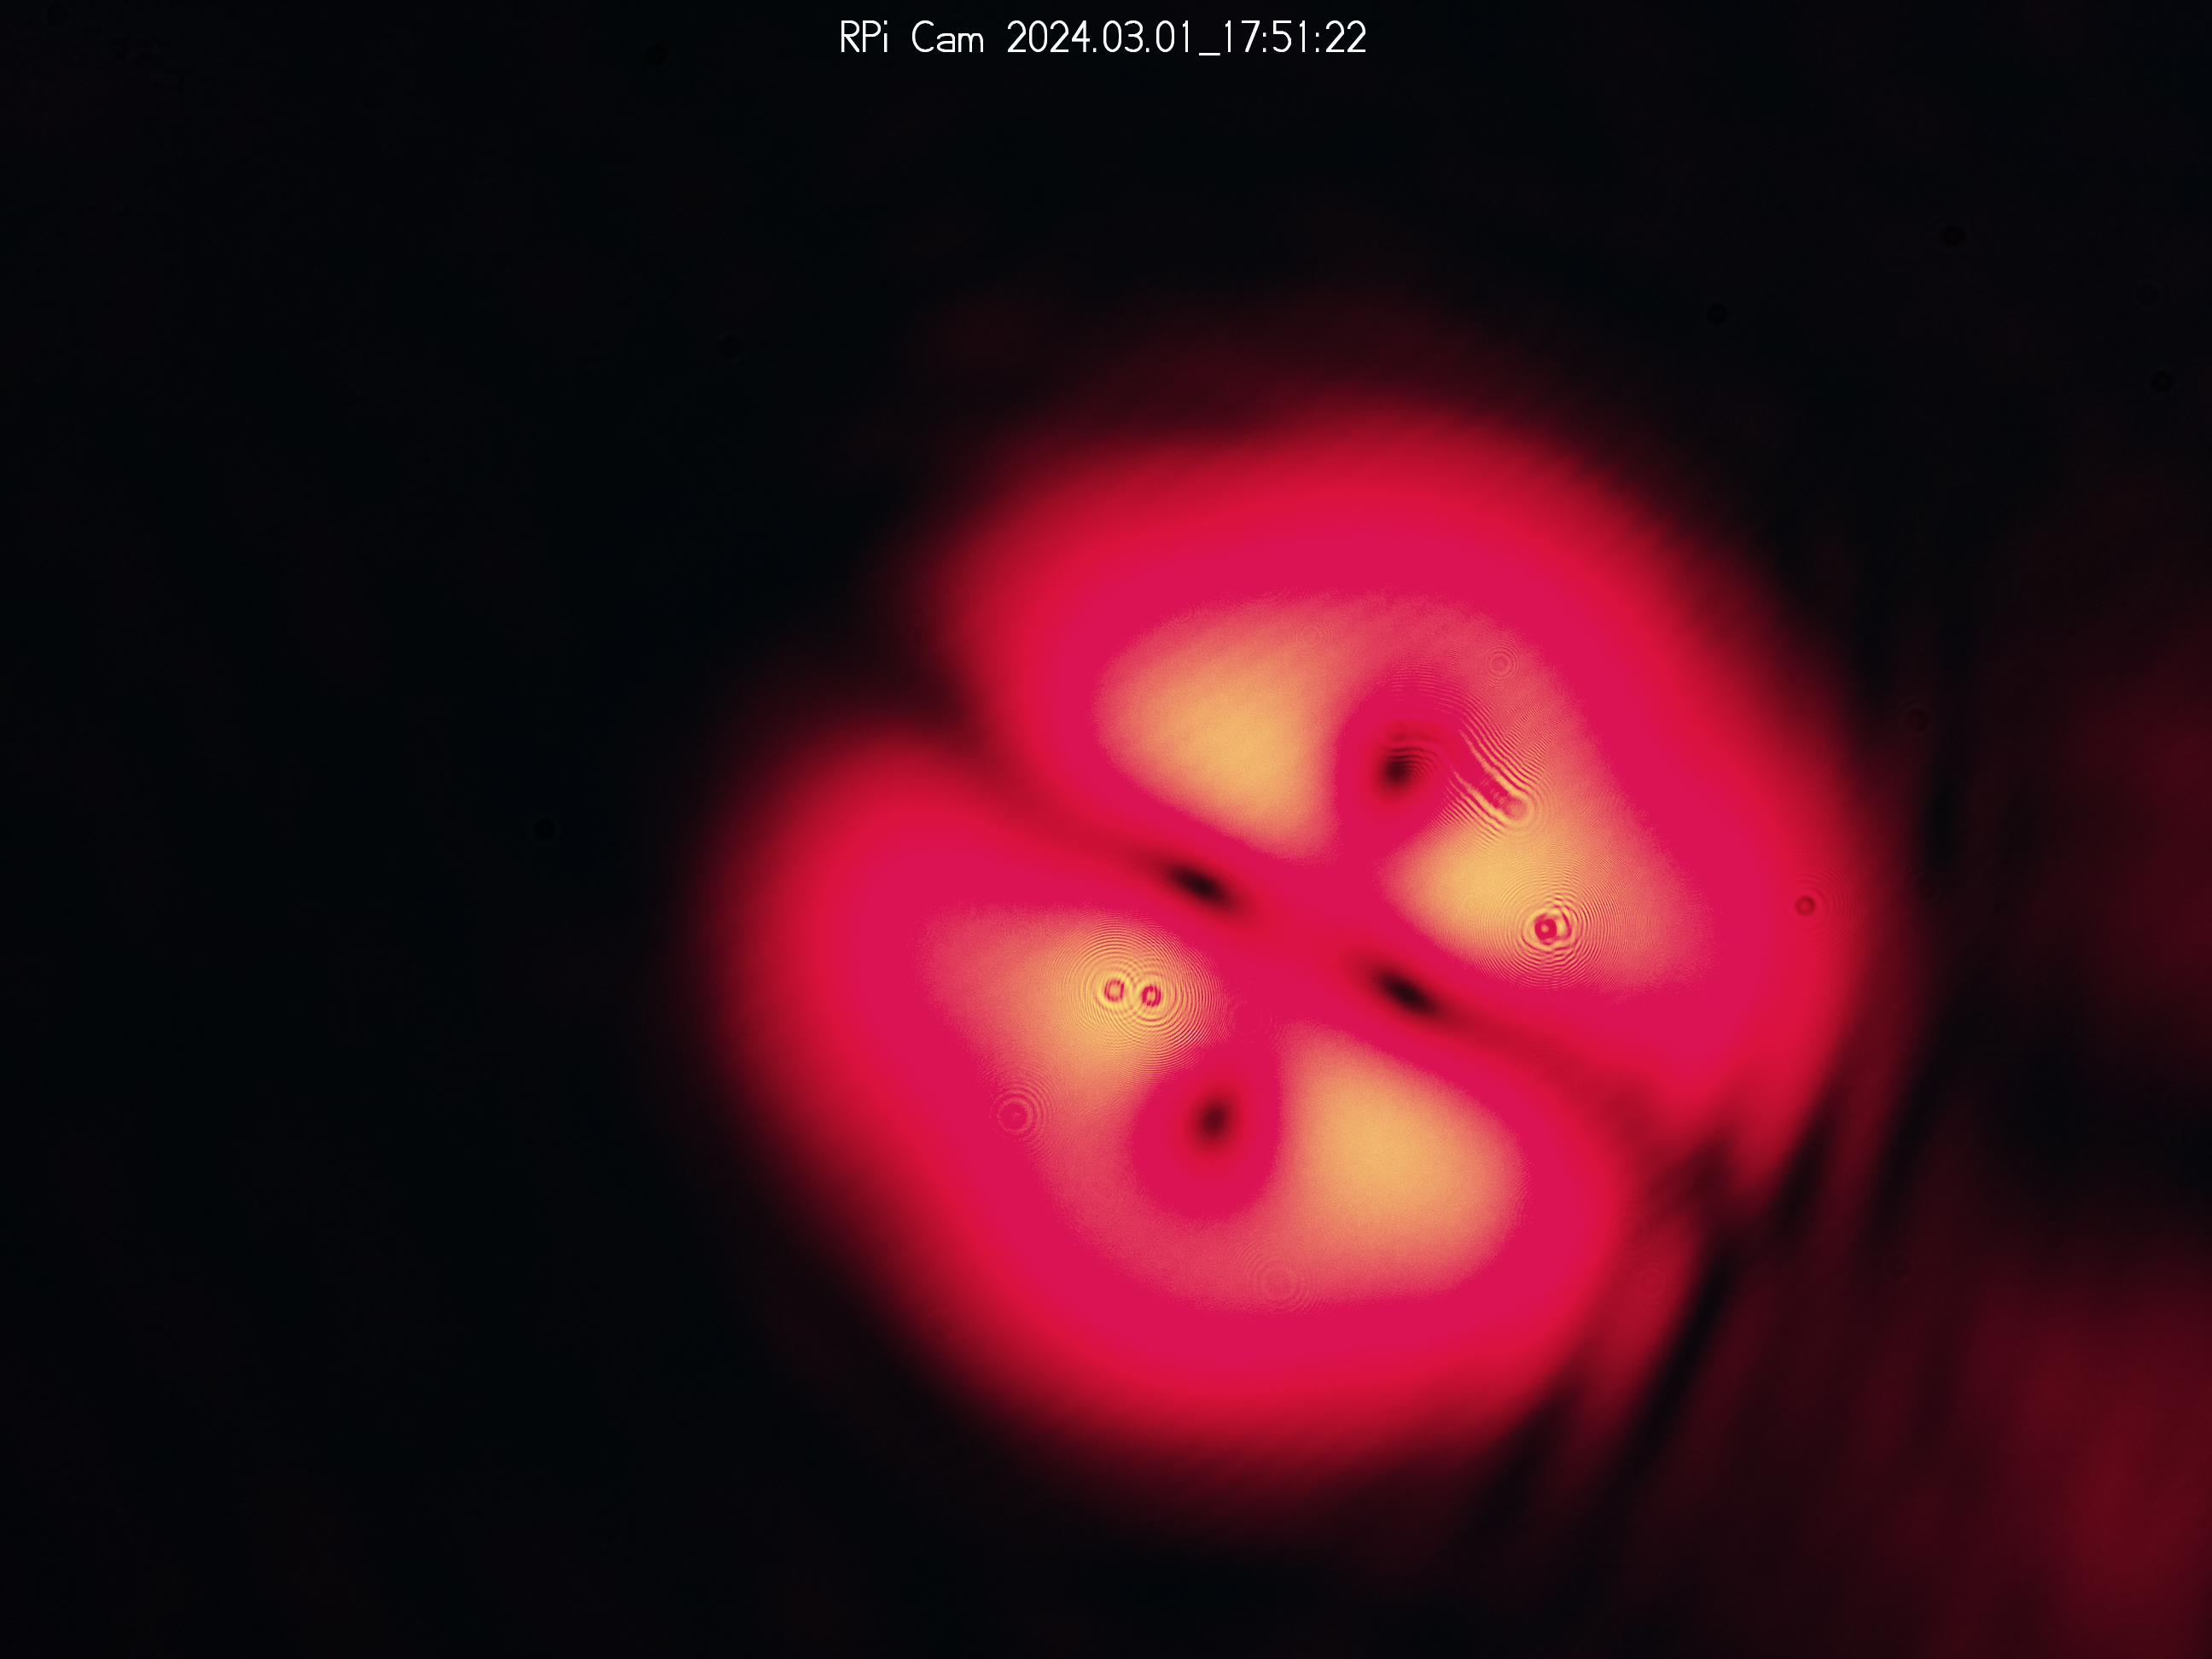
\includegraphics[width=0.3\textwidth]{data/2A/im_0224_20240301_175122.jpg}
    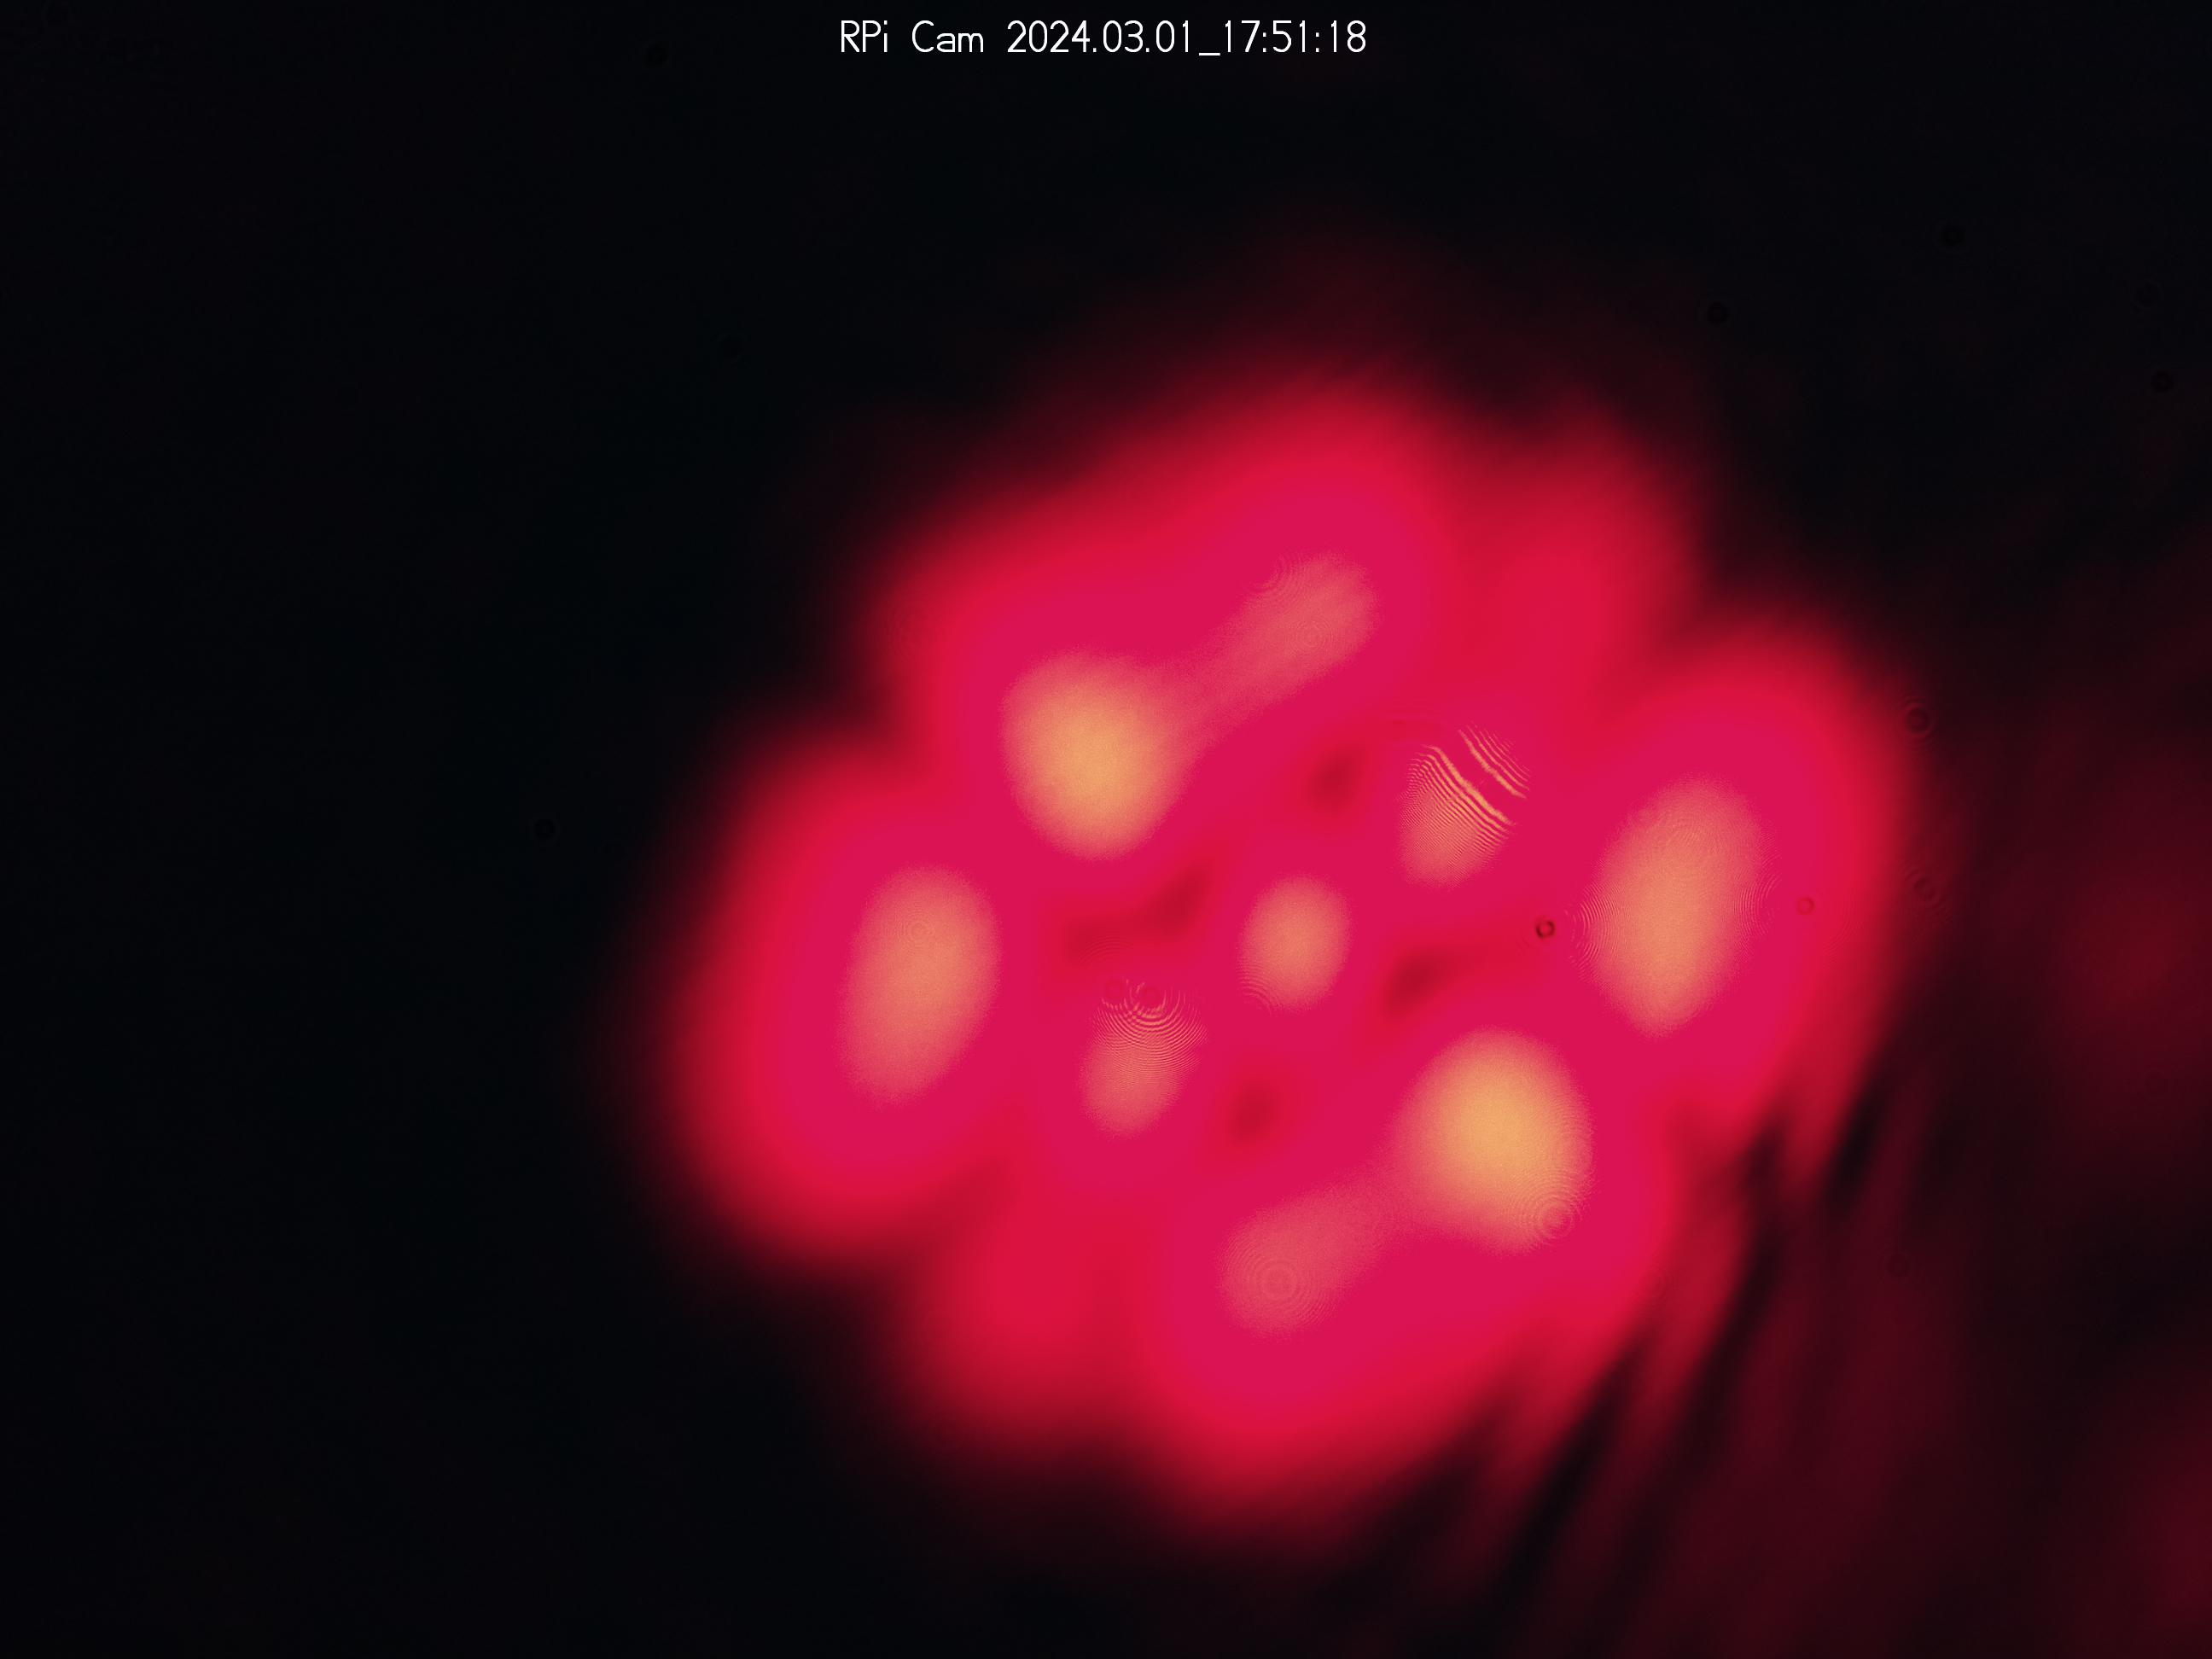
\includegraphics[width=0.3\textwidth]{data/2A/im_0223_20240301_175118.jpg}
    \caption{Selection of mode profiles seen. Left is TEM$_{00}$, middle is TEM$_{11}$ and right is TEM$_{22}$, all Hermite-Gaussian. Especially the TEM$_{22}$ features are fairly blurry, this could either be from interference with other nodes, or just the focus in the camera not being perfectly set up. All of these pictures were taken with a cavity length of 36.5cm.}
    \label{fig:2A}
\end{figure}

\noindent \textcolor{red}{2.3.2B.} See figure \ref{fig:2B}. We started with the TEM$_{22}$ mode, and as can be seen in the figure the modes decreased in complexity until we reached the TEM$_{00}$ mode. This can be explained by the nature of stimulated emission. When a light passes through the HeNe and causes stimulated emission, the resulting photon is in the exact same mode as the first. Therefore if any light is blocked during lasing, this causes an exponential suppression of 

\end{document}
